\begin{figure}[H]
    \centering
    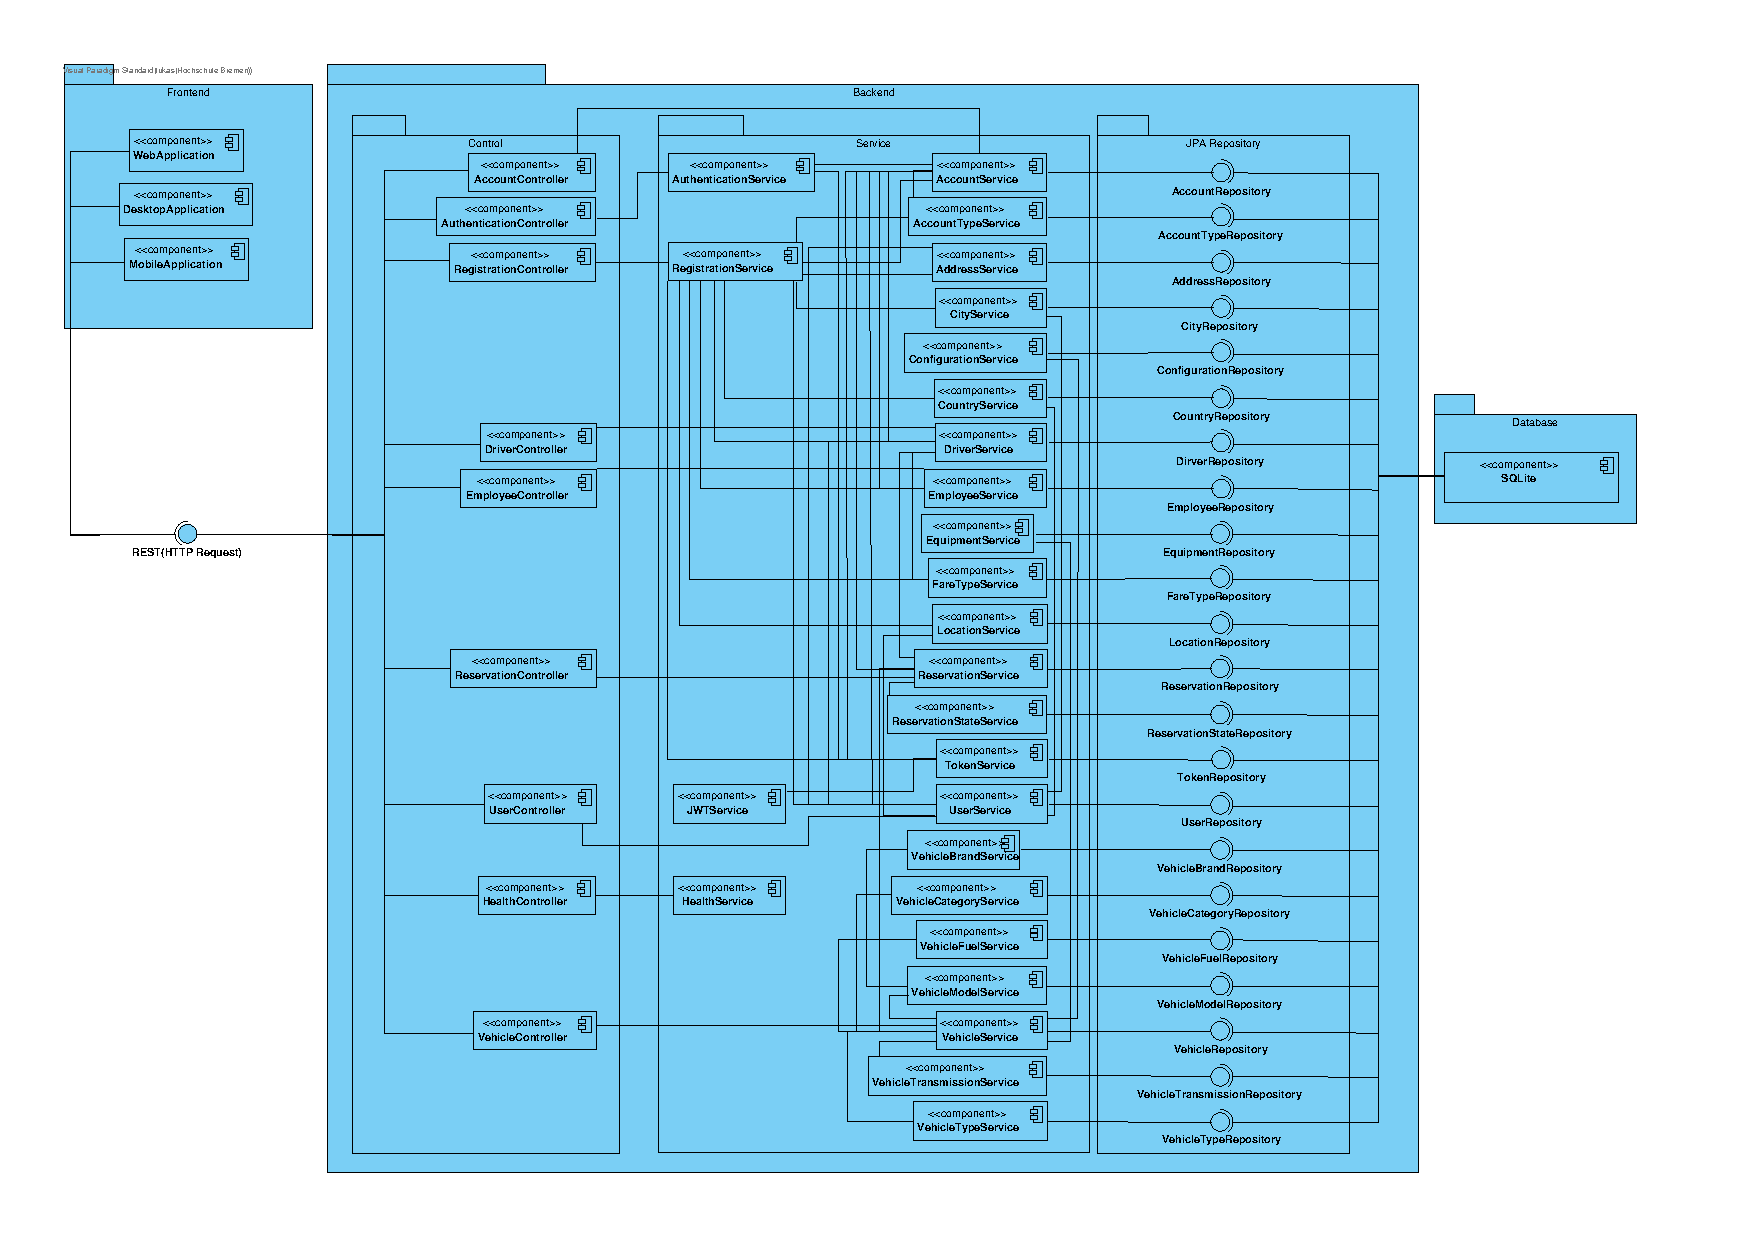
\includegraphics[width = \textwidth]{pictures/fastlane_komponentendiagramm}
    \caption{Komponentendiagramm}
    \label{fig:komponentendiagramm}
\end{figure}
\clearpage
Das Gesamtsystem kann in drei Packages unterteilt werden, um eine bessere Übersicht zu gewährleisten:
\begin{enumerate}
    \item Das Frontend wurde mit Flutter erstellt und umfasst die Web-Anwendung, die Desktop-App und die Mobile-App.
    Diese können über HTTP-Anfragen mit dem Backend kommunizieren.
    \item Das Backend wurde mithilfe von Java und dem Spring Framework entwickelt.
    Es ist in drei kleinere Packages unterteilt:
    \begin{itemize}
        \item Control: Hier befinden sich die Schnittstellendefinitionen für die HTTP-Anfragen.
        Die Controller rufen entsprechende Methoden in den Services auf, um die eingehenden Anfragen zu verarbeiten.
        \item Service: Die Services validieren die Anfragen und können bei Bedarf über die JPA Repositories
        auf die Datenbank zugreifen, um die erforderliche Logik umzusetzen.
        \item JPA Repository: Diese Repositories dienen als Interfaces für den Zugriff auf die SQLite Datenbank.
        Sie sind direkt mit der Datenbank verbunden und ermöglichen das Speichern, Abrufen und Bearbeiten von Daten.
    \end{itemize}
    \item Die Datenbank, welche unter SQLite läuft.
\end{enumerate}

Zusätzlich werden die Verbindungen zwischen den Services dargestellt, da diese auch untereinander kommunizieren.
Beispielsweise ist der \enquote{RegistrationService} mit dem \enquote{AccountService} verbunden, da bei der
Registrierung ein Account erstellt werden muss.